\documentclass{amsart}
\usepackage{amsmath, amsthm, amssymb}
\usepackage{tikz}
\usetikzlibrary{arrows.meta}

\begin{document}

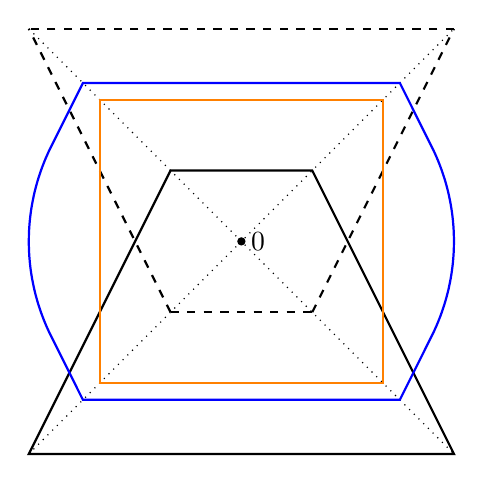
\begin{tikzpicture}[scale=0.9]
\def\p{2}
\def\q{1}
\def\x{((3^\p+1)/2)^(1/\p)}
\def\y{((3^\q+1)/2)^(1/\q)}


\draw[dotted] (-3,-3) -- (3,3);
\draw[dotted] (-3,3) -- (3,-3);


\draw[thick] (-3,-3) -- (3,-3) -- (1,1) -- (-1,1) -- cycle;


\draw[dashed,thick] (3,3) -- (-3,3);
\draw[dashed,thick] (-1,-1) -- (-3,3);
\draw[dashed,thick] (-1,-1) -- (1,-1);
\draw[dashed,thick] (1,-1) -- (3,3);


\draw[orange,thick] ({\y},{\y}) -- ({\y},{-\y}) -- ({-\y},{-\y}) -- ({-\y},{\y}) -- cycle;


\draw[blue,thick,variable=\t,samples=100,domain={1/(3^(\p-1)+1)}:{3^(\p-1)/(3^(\p-1)+1)}]
		plot	(	{3 / (2^(1/\p) * (\t^(\p/(\p-1))+(1-\t)^(\p/(\p-1)))^((\p-1)/\p))},
				{(6 * \t - 3) / (2^(1/\p) * (\t^(\p/(\p-1))+(1-\t)^(\p/(\p-1)))^((\p-1)/\p))}	)
	--	({\x},{\x})
	--	({-\x},{\x})
	--	plot	(	{-3 / (2^(1/\p) * (\t^(\p/(\p-1))+(1-\t)^(\p/(\p-1)))^((\p-1)/\p))},
				{(3 - 6 * \t) / (2^(1/\p) * (\t^(\p/(\p-1))+(1-\t)^(\p/(\p-1)))^((\p-1)/\p))}	)
	--	({-\x},{-\x})
	--	({\x},{-\x})
	--	cycle;


\fill (0,0) circle [radius=1.67pt] node[anchor=west] {0};
\end{tikzpicture}

\end{document}